\begin{frame}
  \begin{PointSix}{Learning Goals}
    \small
    \alert{Learning goals today:}
    \begin{itemize}
      \item Understand that gravity methods map sub-surface density variability
      \item Understand the gravitational force, its potential field, and one underlying measurement principle.
      \item Understand the Earth's geoid and reference ellipsoid
    \end{itemize}
  \end{PointSix}
  \end{frame}

\begin{frame}
  \begin{PointSix}{Example: Global variability}
      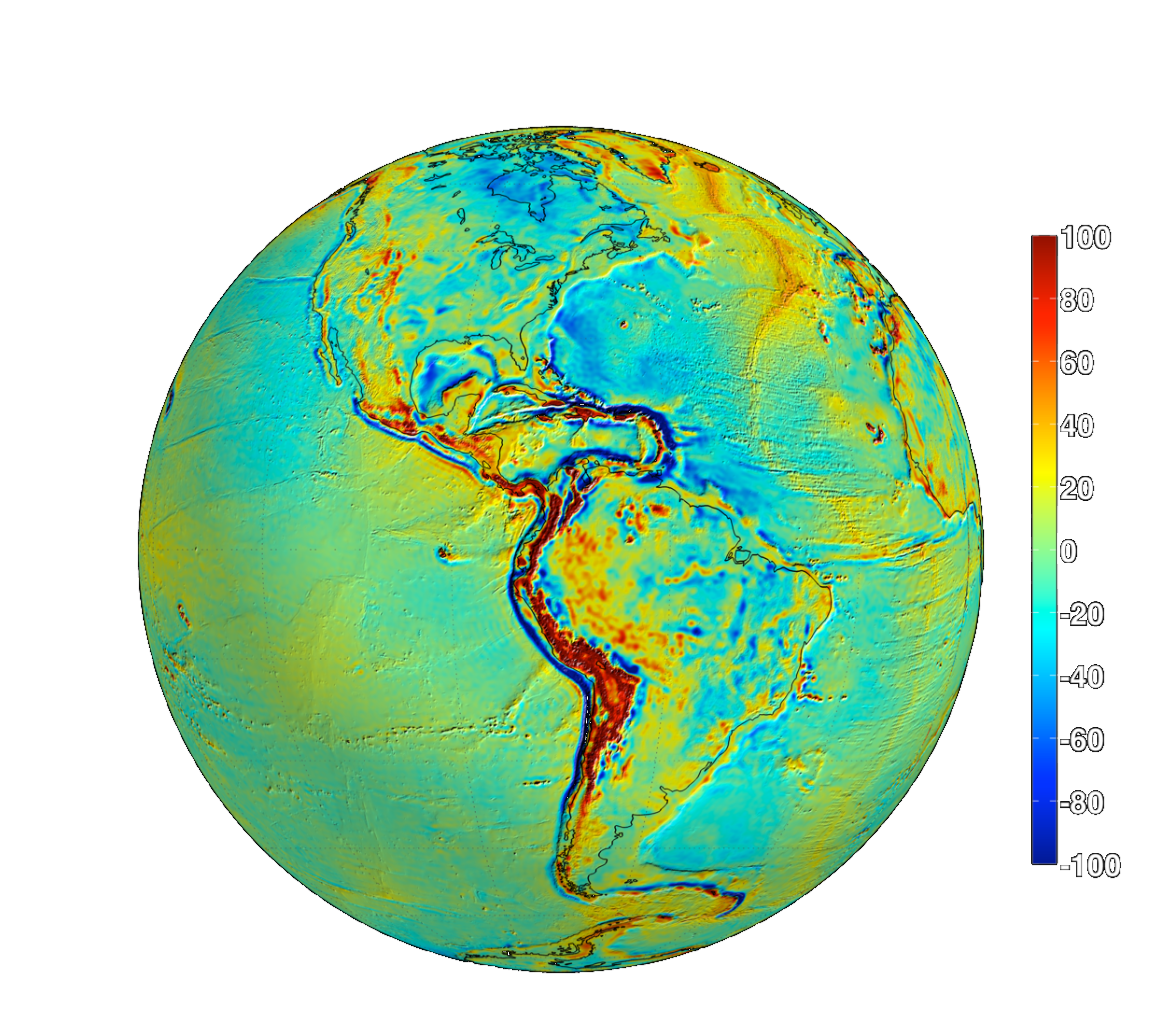
\includegraphics[width=0.99\textwidth]{Figures/Gravity/Exported/Grace_JPLCaltect_FODT10_WithoutPeople.png}
  \end{PointSix}
\end{frame}

\begin{frame}
  \begin{PointSix}{Example: Global variability}
  \centering
  \small Your mass is constant but your weight is not.
  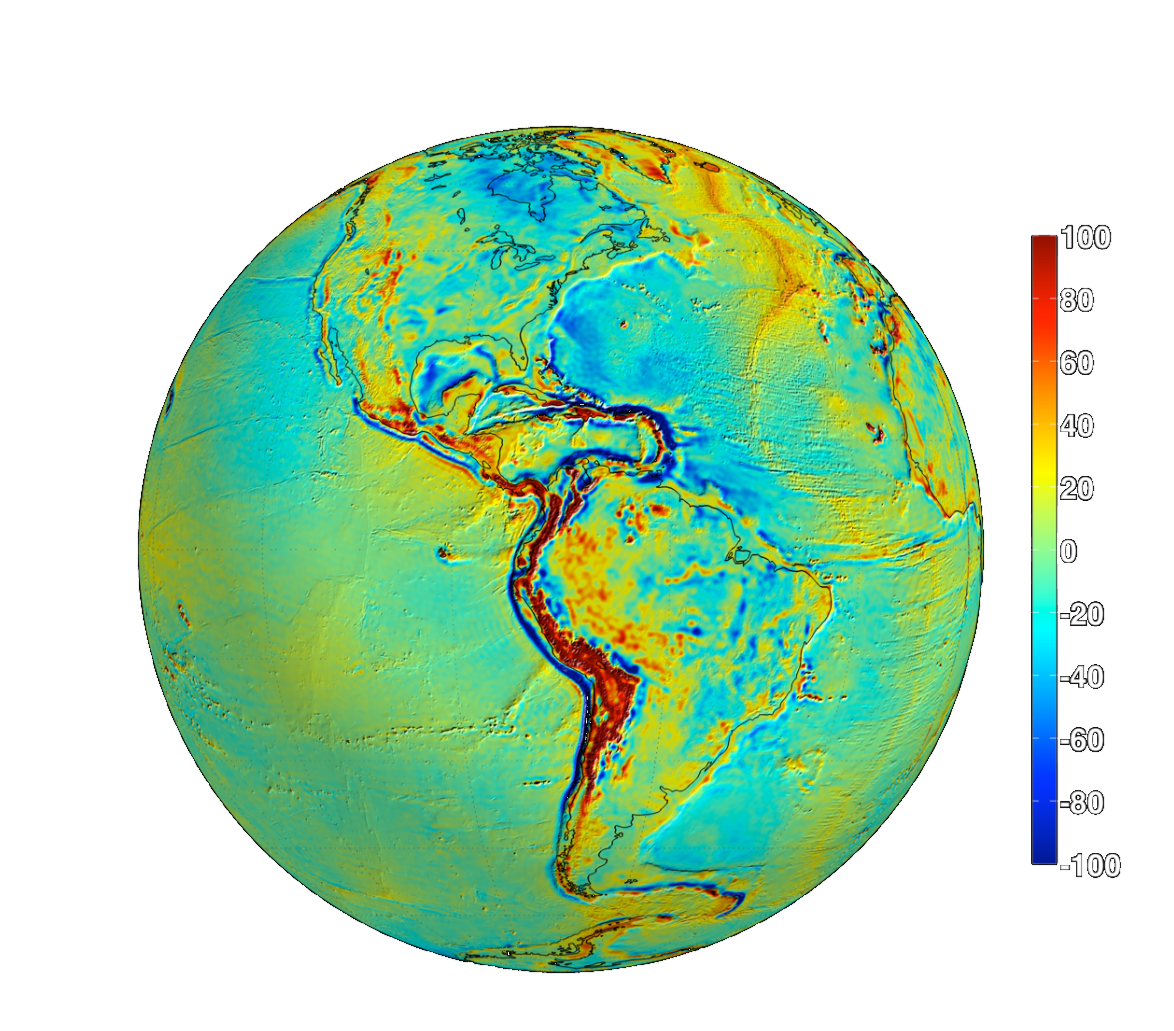
\includegraphics[width=0.99\textwidth]{Figures/Gravity/Exported/Grace_JPLCaltect_FODT10_WithPeople.png}
  \end{PointSix}
\end{frame}


\begin{frame}
\begin{ThreeCols}{What is a force?}{
  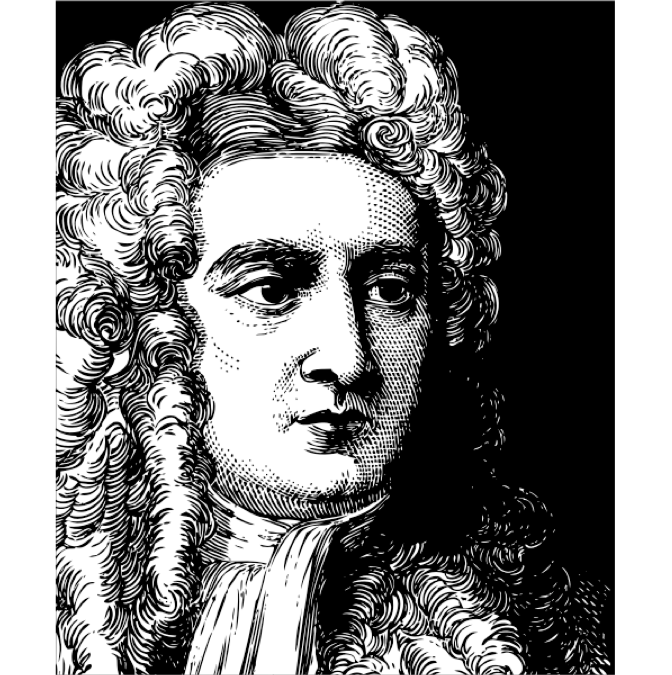
\includegraphics[width=0.8\textwidth]{Figures/Gravity/Exported/Newton_PD_GJohnson.png} \centering \tiny [Newton (1642-1726) / G. Johnson.]}
  \scalebox{1.5}{%
      $
      \vec{F} = m \vec{g}
      $
  }
  \scalebox{0.6}{\parbox{\linewidth}{
      \begin{align*}
      &\vec{F}:\,\text{Force}\,(\text{N};\,\text{kg}\,\text{m}\,\text{s}^{-2})\\
      &\vec{g}:\,\text{Acceleration}\,(\text{m}\,\text{s}^{-2})\\
      &\text{m}:\,\text{Mass (kg)}
      \end{align*}
  }}
\end{ThreeCols}
\end{frame}

\begin{frame}
  \begin{ThreeCols}{The gravitational force}{
      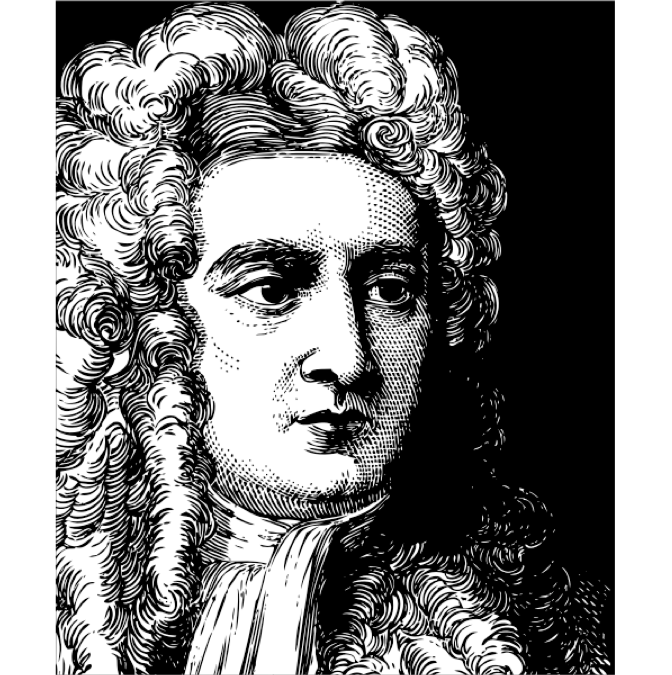
\includegraphics[width=0.8\textwidth]{Figures/Gravity/Exported/Newton_PD_GJohnson.png} \centering \tiny [Newton (1642-1726) / G. Johnson.]}
      \scalebox{1.5}{%
          $
          \vec{F} = G\frac{mM}{r^2}\hat{r}
          $
      }
      \scalebox{0.6}{\parbox{\linewidth}{
          \begin{align*}
          &G=6.674 \cdot 10^{-11}\,\text{(}\,m^3 kg^{-1} s^{-2}\text{)}\\
          &\hat{r}:\,\text{unit vector}\\
          &r:\,\text{distance between point masses}
          \end{align*}
      }}
      \begin{tikzpicture}
          \coordinate (A) at (1,2);
          \coordinate (B) at (2,4);

          \draw [fill=white] (A) circle (8pt) node [left,xshift=-0.5cm] {M};
          \draw [fill=white] (B) circle (4pt) node [left,xshift=-0.5cm] {m};


          \draw[-latex,thick,Karminrot,->] (A) -- (B) node[midway,left,rotate=0] {$r$};
          \draw [-latex,thick, Karminrot] (B) -- (A);
          \end{tikzpicture}
  \end{ThreeCols}
  \end{frame}

  \begin{frame}
      \begin{PointSix}{Example: The gravitational constant}
          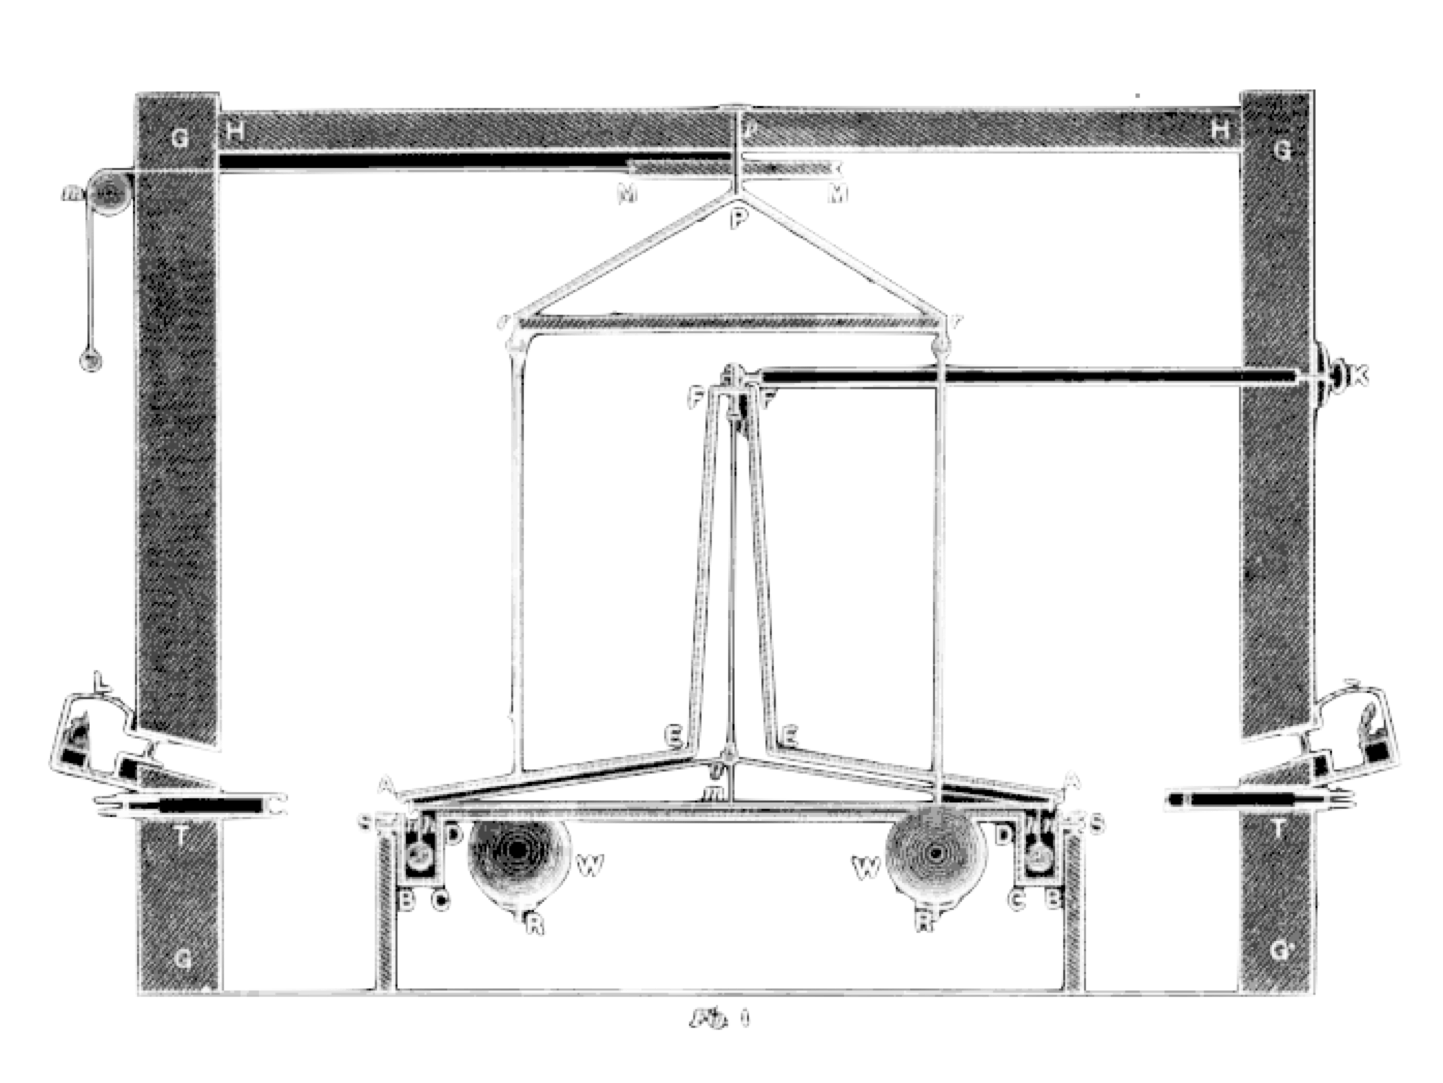
\includegraphics[width=0.99\textwidth]{Figures/Gravity/Exported/Cavendish_PNAS1798.png}
          \centering
          \tiny Cavnedish, PNAS, 1798
      \end{PointSix}
  \end{frame}
  \begin{frame}
      \begin{PointSix}{Example: The gravitational constant}
          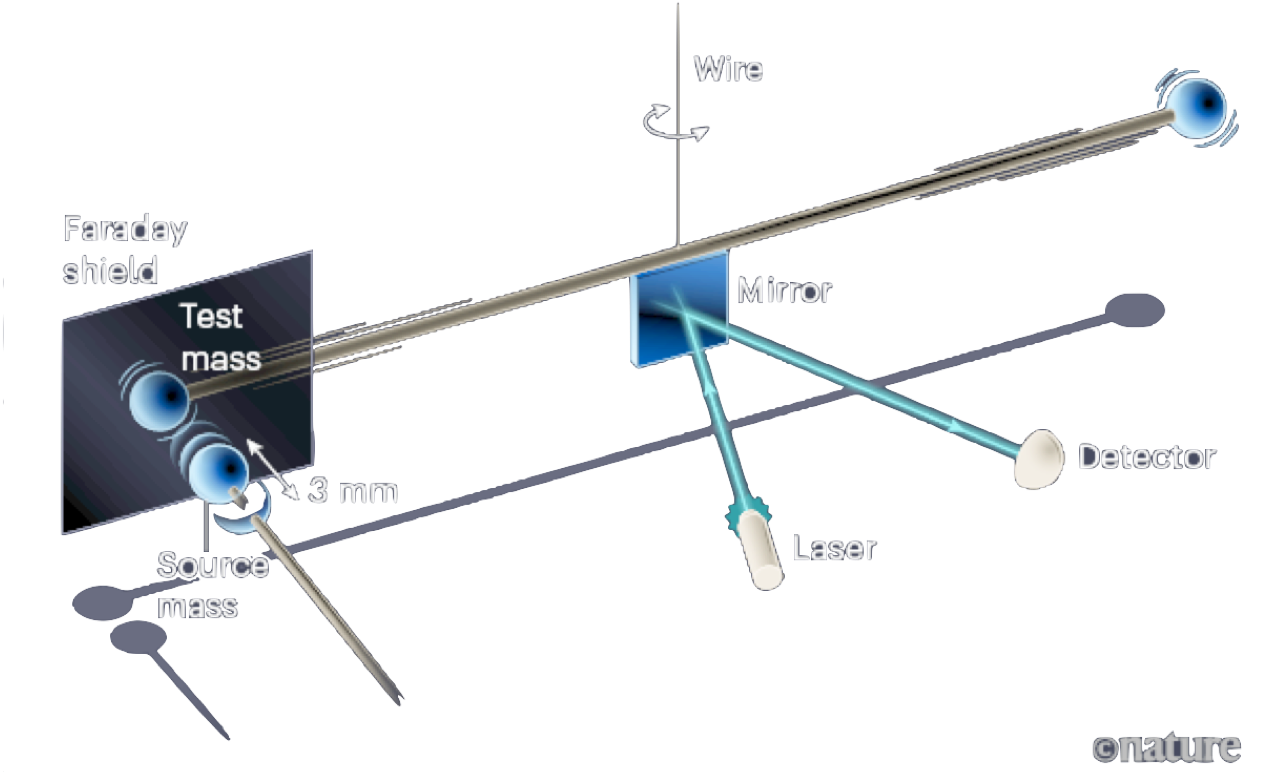
\includegraphics[width=0.99\textwidth]{Figures/Gravity/Exported/MeasuringG_Westphal_Nature2021.png}
          \centering
          \tiny Westphal et al., Nature, 2021\\
          \small G is the worst known constant in physics. Why?
      \end{PointSix}
  \end{frame}

  \begin{frame}
    \begin{PointSix}{Example: Measuring acceleration}
      \begin{minipage}[t]{0.3\textwidth}
       % 
\includegraphics[width=\textwidth]{Figures/General/ScarySmiley_Kindpng.png}
        \end{minipage}\begin{minipage}[]{0.7\textwidth}
      \centering
      \begin{align*}
      &\vec{F} = m \vec{g} \\
      &\vec{F} = G\frac{mM}{r^2}\hat{r} \\
    %  &\rightarrow \vec{g} = G\frac{M}{r^2}\hat{r} \\
    %  &\rightarrow \frac{d^2\vec{x}}{dt^2} = G\frac{M}{r^2}\hat{r} \\
      \end{align*}
      \end{minipage}
      \centering
   %   \small  This is a differential equation.
    \end{PointSix}
    \end{frame}


\begin{frame}
  \begin{PointSix}{Example: Measuring acceleration}
    \begin{minipage}[t]{0.3\textwidth}
      
\includegraphics[width=\textwidth]{Figures/General/ScarySmiley_Kindpng.png}
      \end{minipage}\begin{minipage}[]{0.7\textwidth}
    \centering
    \begin{align*}
    &\vec{F} = m \vec{g} \\
    &\vec{F} = G\frac{mM}{r^2}\hat{r} \\
    &\rightarrow \vec{g} = G\frac{M}{r^2}\hat{r} \\
    &\rightarrow \frac{d^2\vec{x}}{dt^2} = G\frac{M}{r^2}\hat{r} \\
    \end{align*}
    \end{minipage}
    \centering
    \small  This is a differential equation.
  \end{PointSix}
  \end{frame}

\begin{frame}
\begin{PointSix}{Example: Measuring acceleration}
  \begin{minipage}[t]{0.3\textwidth}
    
\includegraphics[width=\textwidth]{Figures/General/IcandothisSmiley_Kindpng.png}
    \end{minipage}\begin{minipage}[]{0.7\textwidth}
  \centering
  \begin{align*}
  &\frac{d^2\vec{x}}{dt^2} = G\frac{M}{R_E^2} \approx const. \\
  \end{align*}
\end{minipage}
 % \centering
 \small
  At the Earth's surface ($R_E$) g is close to constant and only vertical. (Later we will see that none of this is quite true).

\end{PointSix}
\end{frame}

\begin{frame}
  \begin{PointSix}{Example: Measuring acceleration}
  \begin{tikzpicture}
      \begin{axis}[
        rdstyle,
        xlabel=time (s),
        ylabel={$g (m s^{-2})$},
        xmin=0,
        xmax=10,
        xtick={0,2,...,10},
        color=white,
        width=9cm,
      ]
        \addplot[domain=0:10,samples=10,color=Karminrot,line width=0.5mm] {x*0 +9.81};
        \node[] at (axis cs: 5,11) {$g = \frac{d^2}{dt^2}x(t)=\frac{GM}{R_e^2}\approx const.$};
      \end{axis}
    \end{tikzpicture}
  \end{PointSix}
\end{frame}

\begin{frame}
  \begin{PointSix}{Example: Measuring acceleration}
  \begin{tikzpicture}
      \begin{axis}[
        rdstyle,
        xlabel=time (s),
        ylabel={$v (m s^{-1})$},
        xmin=0,
        xmax=10,
        xtick={0,2,...,10},
        ytick=9.81,
        yticklabels={$c_1$},
        color=white,
        width=9cm,
      ]
        \addplot[domain=0:10,samples=10,color=Karminrot,line width=0.5mm] {x + 9.81};
        \node[] at (axis cs: 5,20) {$v = \int g dt=\frac{d}{dt}x(t)=\frac{GM}{R_e^2}t+c_1$};
      \end{axis}
    \end{tikzpicture}
  \end{PointSix}
\end{frame}

\begin{frame}
  \begin{PointSix}{Example: Measuring acceleration}
  \begin{tikzpicture}
      \begin{axis}[
        rdstyle,
        xlabel=time (s),
        ylabel={$x (m)$},
        xmin=0,
        xmax=10,
        xtick={0,2,...,10},
        ytick=9.81,
        yticklabels={$c_2$},
        color=white,
        width=9cm,
      ]
        \addplot[domain=0:10,samples=10,color=Karminrot,line width=0.5mm] {x^2 + 10};
        \node[] at (axis cs: 5,100) {$x(t) = \int v(t) dt=\frac{GM}{2R_e^2}t^2+c_1t+c_2$};
      \end{axis}
    \end{tikzpicture}
  \end{PointSix}
\end{frame}
\begin{frame}

\begin{PointSix}{Example: Measuring acceleration}
     \begin{align*}
       & x(t) = \frac{GM}{2R_e^2}t^2+c_1t+c_2 \\
     \end{align*}
     \small
     \begin{itemize}
      \item Setting, e.g., $c1=0$ (initial velocity) and $c_2=0$ (initial position) is quite convenient.
      \item This is the principal of a free-fall gravimeter.
    \end{itemize}
\end{PointSix}

\end{frame}

\begin{frame}
\begin{PointSix}{Exercises: Group-Work Thursdays}
  \small
  \begin{itemize}
    \item Thanks to the Greeks we know the radius $R_E$ for the Earth. However, its mass was unknown for a while.
    \item Go ahead and determine the mass of the Earth M with your Smartphone!
    \item \alert{There is an important first-order finding in Earth Sciences that you can (re-) discover. Which one?}
  \end{itemize}

\end{PointSix}
\end{frame}

\begin{frame}
\begin{PointSix}{Beyond point masses}
  \begin{tikzpicture}
    \coordinate (A) at (8,0);
    \coordinate (B) at (4,-3.5);
    \coordinate (C) at (5,-3.5);
    \coordinate (D) at (6,-3.5);
    \draw [thick] (0,0.0) -- (8,0.0);
    % drawing the node with shape=rectangle and anchor=center
    \node [draw, Karminrot, thick, shape=rectangle, minimum width=0.25cm, minimum height=0.25cm, anchor=center] at (B) {};
    \draw [->, thick] (0,0.0) -- (B) node[xshift=0.3cm,yshift=0.3cm,midway,left,rotate=-30] {$\vec{r}$};;

    \node[yshift=0.3cm] at (A) {\small Surface};

  \end{tikzpicture}
  $$
    \vec{F} = G\frac{dM}{r^2}\hat{r}
  $$
\small For a small mass dM the point mass approximation holds.
\end{PointSix}

\end{frame}



\begin{frame}
\begin{PointSix}{Beyond point masses}
  \begin{tikzpicture}
    \coordinate (A) at (8,0);
    \coordinate (B) at (4,-3.5);
    \coordinate (C) at (5,-3.5);
    \coordinate (D) at (6,-3.5);
    \draw [thick] (0,0.0) -- (8,0.0);
    % drawing the node with shape=rectangle and anchor=center
    \node [draw, Karminrot, thick, shape=rectangle, minimum width=0.25cm, minimum height=0.25cm, anchor=center] at (B) {};
    \foreach \i in {0,2,...,8}
    {
      \draw [->, thick] (0+\i,0.0) -- (B);
    }
    \node[yshift=0.3cm] at (A) {\small Surface};

  \end{tikzpicture}
  $$
    \vec{F} = G\frac{dM}{r^2}\hat{r}
  $$
  \small Profiling across a sub-surface target results in a gravity anomaly ($\rightarrow$ Exercises).
\end{PointSix}
\end{frame}

\begin{frame}
\begin{PointSix}{Beyond point masses}
  \begin{tikzpicture}
    \coordinate (A) at (8,0);
    \coordinate (B) at (4,-3.5);
    \coordinate (C) at (5,-3.5);
    \coordinate (D) at (6,-3.5);
    \draw [thick] (0,0.0) -- (8,0.0);
    \node[yshift=0.3cm] at (A) {\small Surface};

    \foreach \i in {-2,-1.5,...,2}
    {
      \foreach \j in {0,0.5}
      {
        \node [draw, Karminrot, thick, shape=rectangle, minimum width=0.25cm, minimum height=0.25cm, anchor=center] at (4-\i,-3.5-\j) {};
        \draw [->, thick] (0,0.0) -- (4-\i,-3.5-\j) ;

      }
    }

  \end{tikzpicture}
  $$
  \vec{F}(\vec{r}) = \sum_i G\frac{dM_i}{r_i^2}\hat{r_i}
  $$
  \small For $i$ point masses the effect adds up.
\end{PointSix}
\end{frame}

\begin{frame}
\begin{PointSix}{Beyond point masses}
  \begin{tikzpicture}
    \coordinate (A) at (8,0);
    \coordinate (B) at (4,-3.5);
    \coordinate (C) at (5,-3.5);
    \coordinate (D) at (6,-3.5);
    \draw [thick] (0,0.0) -- (8,0.0);
    \node[yshift=0.3cm] at (A) {\small Surface};

    \foreach \i in {-2,-1.5,...,2}
    {
      \foreach \j in {0,0.5}
      {
        \node [draw, Karminrot, thick, shape=rectangle, minimum width=0.25cm, minimum height=0.25cm, anchor=center] at (4-\i,-3.5-\j) {};
        \draw [->, thick] (2,0.0) -- (4-\i,-3.5-\j) ;

      }
    }
  \end{tikzpicture}
  $$
    \vec{F}(\vec{r}) = \sum G\frac{dM_i}{r_i^2}\hat{r_i}
  $$
\end{PointSix}

\end{frame}

\begin{frame}
\begin{PointSix}{Beyond point masses}
  \begin{tikzpicture}
    \coordinate (A) at (8,0);
    \coordinate (B) at (4,-3.5);
    \coordinate (C) at (5,-3.5);
    \coordinate (D) at (6,-3.5);
    \draw [thick] (0,0.0) -- (8,0.0);
    \node[yshift=0.3cm] at (A) {\small Surface};
    \foreach \i in {-2,-1.5,...,2}
    {
      \foreach \j in {0,0.5}
      {
        \node [draw, Karminrot, thick, shape=rectangle, minimum width=0.25cm, minimum height=0.25cm, anchor=center] at (4-\i,-3.5-\j) {};
        \draw [->, thick] (4,0.0) -- (4-\i,-3.5-\j) ;

      }
    }
  \end{tikzpicture}
  $$
  \vec{F}(\vec{r}) = \sum G\frac{dM_i}{r_i^2}\hat{r_i}
  $$
\end{PointSix}
\end{frame}


\begin{frame}
\begin{PointSix}{Beyond point masses}
  \begin{tikzpicture}
    \coordinate (A) at (8,0);
    \coordinate (B) at (4,-3.5);
    \coordinate (C) at (5,-3.5);
    \coordinate (D) at (6,-3.5);
    \draw [thick] (0,0.0) -- (8,0.0);
    \node[yshift=0.3cm] at (A) {\small Surface};

    \foreach \i in {-2,-1.5,...,2}
    {
      \foreach \j in {0,0.5}
      {
        \node [draw, Karminrot, thick, shape=rectangle, minimum width=0.25cm, minimum height=0.25cm, anchor=center] at (4-\i,-3.5-\j) {};
        \draw [->, thick] (7,0.0) -- (4-\i,-3.5-\j) ;

      }
    }
  \end{tikzpicture}
  $$
  \vec{F}(\vec{r}) = \sum G\frac{dM_i}{r_i^2}\hat{r_i}
  $$
\end{PointSix}
\end{frame}


\begin{frame}
\begin{PointSix}{Beyond point masses}
  \begin{tikzpicture}
    \coordinate (A) at (8,0);
    \coordinate (B) at (4,-3.5);
    \coordinate (C) at (5,-3.5);
    \coordinate (D) at (6,-3.5);
    \draw [thick] (0,0.0) -- (8,0.0);
    \node[yshift=0.3cm] at (A) {\small Surface};
    \node[yshift=-1.8cm,xshift=-4cm] at (A) {$\vec{F}(\vec{r}) = G \int \rho \frac{1}{r^2}\hat{r}dV$};

    %
    \foreach \i in {-2,-1.5,...,2}
    {
      \foreach \j in {0,0.5}
      {
        \node [draw, Karminrot, thick, shape=rectangle, minimum width=0.25cm, minimum height=0.25cm, anchor=center] at (4-\i,-3.5-\j) {};
        %\draw [->, thick] (7,0.0) -- (4-\i,-3.5-\j) ;
      }
    }
    \node [draw, Karminrot, thick, shape=rectangle, minimum width=4.5cm, minimum height=1.25cm, anchor=center] at (4,-3.75) {};
  \end{tikzpicture}

  \only<1>{\small The summation can be replaced by an integration over a volume enclosing a continuous density.}\only<2>{\small The integration is a triple integral. Integration limits and coordinates depend on the viewpoint. Example is a Bouger plate, in general not easy to solve ($\rightarrow$ Exercises).}
    %\only<1>{The summation can be replaced by an integration over a volume enclosing a continuous density.} d $\rho$}\only<2>{Test,}d
\end{PointSix}
\end{frame}

\begin{frame}
\begin{PointSix}{Example: Shell}
  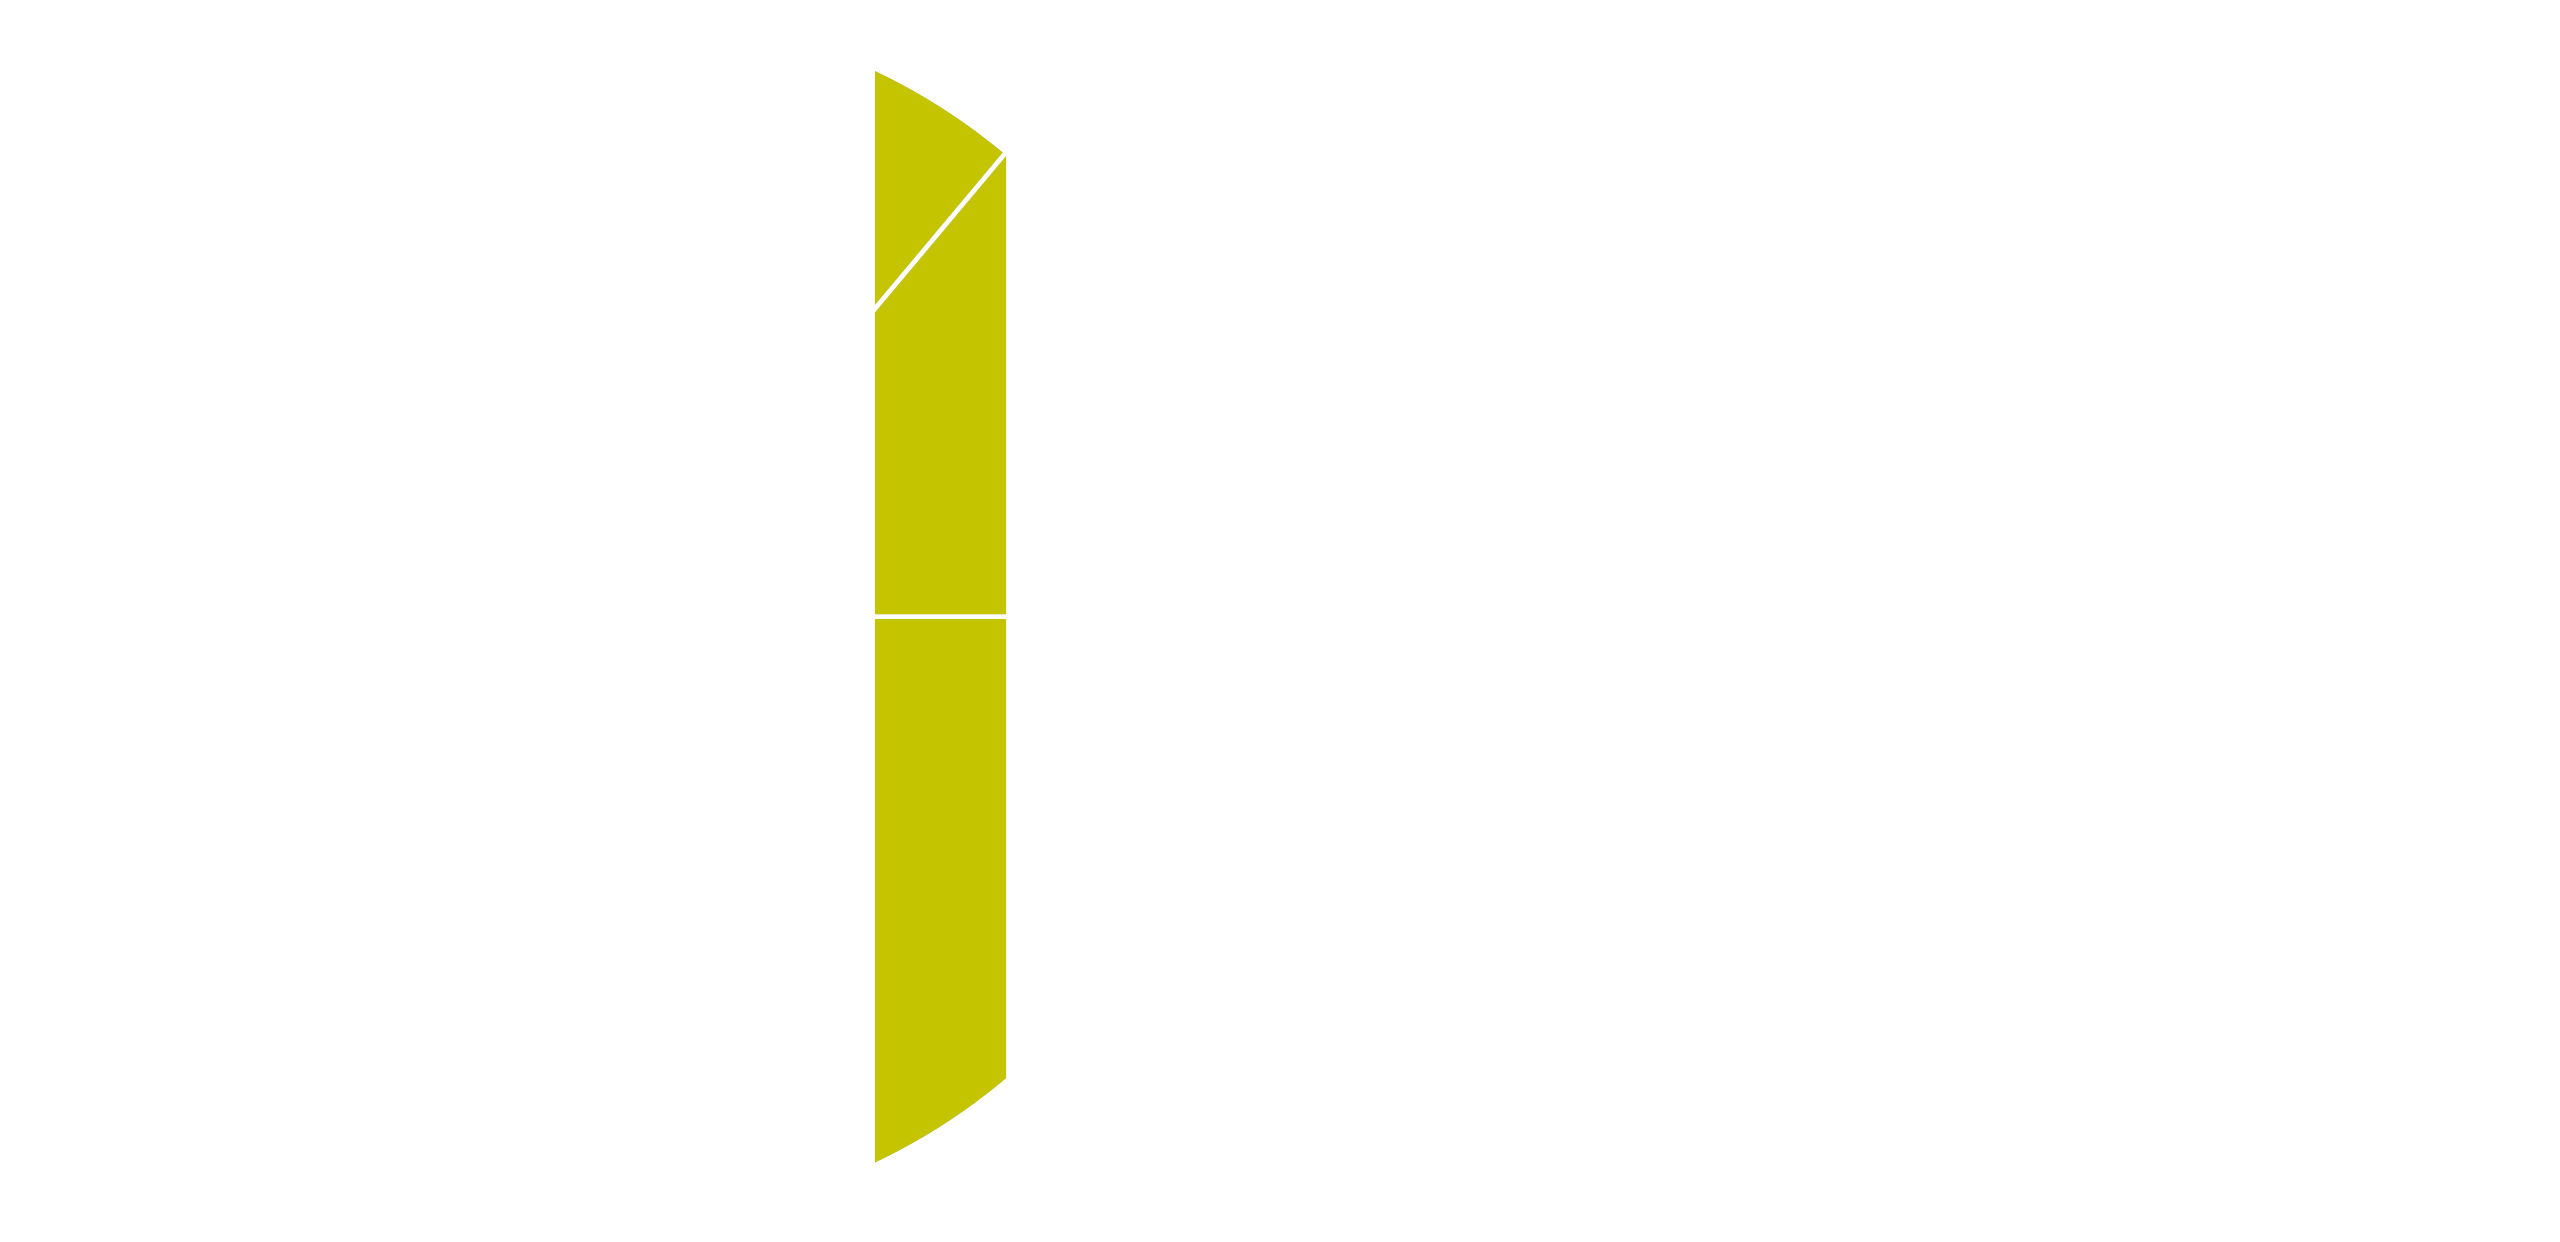
\includegraphics[width=0.99\textwidth]{Figures/Gravity/Exported/Shell-diag_reversed_CCBYSA4_0_Xaonon.png}
  \tiny [Xaononl CC BY-SA 4.0]

  \small Newton's shell theorem solves the volume integral inside and outside spherical objects ($\rightarrow$ Ex.-Discussion)
\end{PointSix}

\end{frame}

\begin{frame}
\begin{PointSix}{Newton's Shell Theorem}
\small
 \begin{itemize}
    \item The field outside a shell is the same as the one from an equivalent point mass
    \item The field inside a shell is zero. Everywhere.
 \end{itemize}
\end{PointSix}
\end{frame}

\begin{frame}
\begin{PointSix}{Other shapes}
 \begin{itemize}
    \item \small There are analytical solutions for other shapes (e.g., Nagy 1966 for Prism).
 \end{itemize}
 \begin{center}
    \begin{tikzpicture}[>=latex,scale=2]

        \pgfmathsetmacro{\x}{1}
        \pgfmathsetmacro{\y}{1}
        \pgfmathsetmacro{\z}{1.5}
        \path (0,0,\y) coordinate (A) (\x,0,\y) coordinate (B) (\x,0,0) coordinate (C) (0,0,0)
        coordinate (D) (0,\z,\y) coordinate (E) (\x,\z,\y) coordinate (F) (\x,\z,0) coordinate (G)
        (0,\z,0) coordinate (H);
        \draw [thick] (-2,1.8) -- (3,1.8);
        \draw (A)--(B)--(C)--(G)--(F)--(B) (A)--(E)--(F)--(G)--(H)--(E);
        \draw (A)--(D)--(C) (D)--(H);
        \node[yshift=-0.3cm] at (2,1.8) {\small Surface};
        \draw[thin,|<->|] ($(A)+(0,-4pt)$) -- node[below]{x}($(B)+(0,-4pt)$);
        \draw[thin,|<->|] ($(B)+(-45:4pt)$) -- node[below,sloped]{y}($(C)+(-45:4pt)$);
        \draw[thin,|<->|] ($(C)+(4pt,0)$) -- node[below,sloped]{z}($(G)+(4pt,0)$);

    \end{tikzpicture}
\end{center}
\end{PointSix}
\end{frame}


\begin{frame}
\begin{PointSix}{Numerical forward modelling ($\rightarrow$ Ex)}
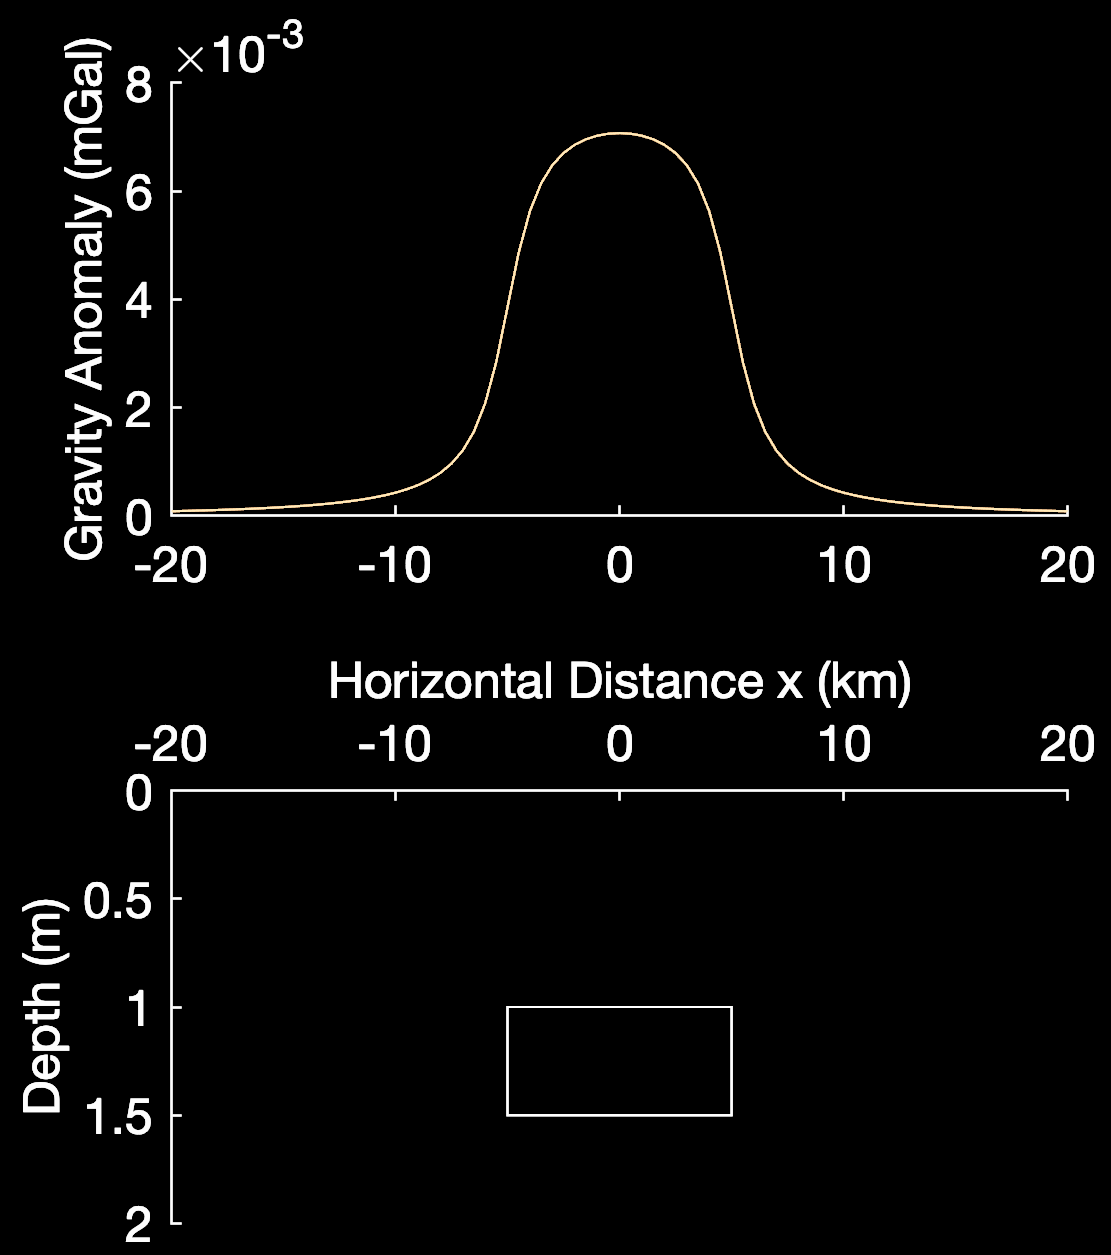
\includegraphics[width=0.8\textwidth]{Figures/Gravity/Exported/ForwardModelPrismReversed.png}
\end{PointSix}
\end{frame}



\begin{frame}
  \begin{PointSix}{Vector fields}
    \centering
    $
    \vec{g} = G\frac{M}{r^2}\hat{r}
    $
    \begin{center}
    \scalebox{0.85}{
        \begin{tikzpicture}
          \begin{axis}[
              xmin = -4, xmax = 4,
              ymin = -4, ymax = 4,
              zmin = 0, zmax = 1,
              axis equal image,
              xtick distance = 20,
              ytick distance = 20,
              view = {0}{90},
              scale = 1.25,
            % title = {\bf Vector Field $F = [-y,x]$},
              height=7cm,
            % xlabel = {$x$},
            % ylabel = {$y$},
              colormap/viridis,
            % colorbar,
            % colorbar style = {
            %     ylabel = {Vector Length}
            % }
            hide x axis,
            hide y axis,
          ]
          \addplot3[
                  point meta = {sqrt(x^2+y^2)},
                  quiver = {
                      u = {-x/sqrt(x^2+y^2)^2},
                      v = {-y/sqrt(x^2+y^2)^2},
                      scale arrows = 0.7,
                  },
                  quiver/colored = {mapped color},
                  -stealth,
                  samples = 10,
                  domain = -4:4,
                  domain y = -4:4,
                  ] {0};
          \end{axis}
          \draw [fill=white] (3.4,3.4) circle (0.5cm);
        \end{tikzpicture}
    }
      \end{center}

  \end{PointSix}
 \end{frame}

 \begin{frame}
  \begin{PointSix}{Potential Field}
    \centering
    $
    \vec{g} = G\frac{M}{r^2}\hat{r}
    $
    \begin{center}
    \scalebox{0.85}{
        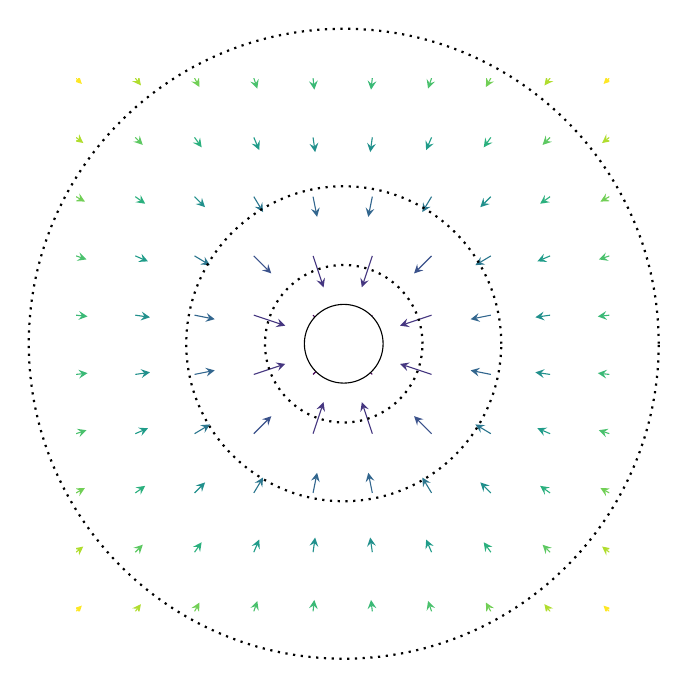
\begin{tikzpicture}
          \begin{axis}[
              xmin = -4, xmax = 4,
              ymin = -4, ymax = 4,
              zmin = 0, zmax = 1,
              axis equal image,
              xtick distance = 20,
              ytick distance = 20,
              view = {0}{90},
              scale = 1.25,
            % title = {\bf Vector Field $F = [-y,x]$},
              height=7cm,
            % xlabel = {$x$},
            % ylabel = {$y$},
              colormap/viridis,
            % colorbar,
            % colorbar style = {
            %     ylabel = {Vector Length}
            % }
            hide x axis,
            hide y axis,
          ]
          \addplot3[
                  point meta = {sqrt(x^2+y^2)},
                  quiver = {
                      u = {-x/sqrt(x^2+y^2)^2},
                      v = {-y/sqrt(x^2+y^2)^2},
                      scale arrows = 0.7,
                  },
                  quiver/colored = {mapped color},
                  -stealth,
                  samples = 10,
                  domain = -4:4,
                  domain y = -4:4,
                  ] {0};

              %For some reason gnuplot does not work.
              % \addplot3[contour gnuplot={number=50,labels=false, draw color=blue},thick,]
              % {
              %   abs(((1)/sqrt((x-2)^2+y^2) - (1)/sqrt((x+2)^2+y^2)))<4 ? ((1)/sqrt((x-2)^2+y^2) - (1)/sqrt((x+2)^2+y^2)) : NaN
              % };
          \end{axis}
          \draw [fill=white] (3.4,3.4) circle (0.5cm);
          \draw [dotted, thick] (3.4,3.4) circle (1.cm);
          \draw [dotted, thick] (3.4,3.4) circle (2.cm);
          \draw [dotted, thick] (3.4,3.4) circle (4.cm);
        \end{tikzpicture}
      }
      \end{center}

  \end{PointSix}
 \end{frame}

 \begin{frame}
  \begin{PointSix}{Potential Field}
    \centering
    \small What is the amount of work required?
    \begin{center}
    \scalebox{0.85}{
        \begin{tikzpicture}
          \begin{axis}[
              xmin = -4, xmax = 4,
              ymin = -4, ymax = 4,
              zmin = 0, zmax = 1,
              axis equal image,
              xtick distance = 20,
              ytick distance = 20,
              view = {0}{90},
              scale = 1.25,
            % title = {\bf Vector Field $F = [-y,x]$},
              height=7cm,
            % xlabel = {$x$},
            % ylabel = {$y$},
              colormap/viridis,
            % colorbar,
            % colorbar style = {
            %     ylabel = {Vector Length}
            % }
            hide x axis,
            hide y axis,
          ]
          \addplot3[
                  point meta = {sqrt(x^2+y^2)},
                  quiver = {
                      u = {-x/sqrt(x^2+y^2)^2},
                      v = {-y/sqrt(x^2+y^2)^2},
                      scale arrows = 0.7,
                  },
                  quiver/colored = {mapped color},
                  -stealth,
                  samples = 10,
                  domain = -4:4,
                  domain y = -4:4,
                  ] {0};

              %For some reason gnuplot does not work.
              % \addplot3[contour gnuplot={number=50,labels=false, draw color=blue},thick,]
              % {
              %   abs(((1)/sqrt((x-2)^2+y^2) - (1)/sqrt((x+2)^2+y^2)))<4 ? ((1)/sqrt((x-2)^2+y^2) - (1)/sqrt((x+2)^2+y^2)) : NaN
              % };
          \end{axis}
          \draw [fill=white] (3.4,3.4) circle (0.5cm);
          \draw [dotted, thick] (3.4,3.4) circle (1.cm);
          \draw [dotted, thick] (3.4,3.4) circle (2.cm);
          \draw [dotted, thick] (3.4,3.4) circle (4.cm);
          \draw[-latex,thick,Karminrot,->] (4.1,4.1) -- (6.2,6.2) node[midway,left,rotate=0] {$r$};
        \end{tikzpicture}
    }
      \end{center}

  \end{PointSix}
 \end{frame}


\begin{frame}
  \begin{PointSix}{Potential Fields}
    \begin{align*}
      U(r) &=& -\int_{\infty}^r \vec{g}d{\vec{r}} \\
           &=& -\int_{\infty}^r gd{r} \\
           &=& -GM\int_{\infty}^r \frac{1}{r^2}d{r} \\
           &=& -GM \left[ -\frac{1}{r}\right]_{\infty}^r \\
           &=& GM\frac{1}{r}
    \end{align*}
    Potential for a point mass.
  \end{PointSix}
\end{frame}

\begin{frame}
  \begin{PointSix}{Potential Fields}
    \begin{align*}
      \vec{g}(r) = -\nabla U(r)
    \end{align*}
    \small
    \begin{itemize}
      \item It is sometimes easier to calculate the potential of an anomaly and to infer the acceleration via the gradient.
      \item Equipotential lines are perpendicular to the field direction.
      \item Equipotential lines are in general NOT lines of equal field strength (cf. with down-hill slope force in landscape)
    \end{itemize}
  \end{PointSix}
\end{frame}


\begin{frame}
\begin{PointSix}{Gravitational field of a spherical Earth}
  \small The Earth's rotation minimizes gravitational acceleration at the equator. At the poles it does nothing.
  \begin{center}
  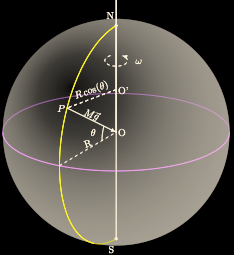
\includegraphics[width=0.6\textwidth]{Figures/Gravity/Exported/GravityFieldEarthRotation_Reversed.png}
  \end{center}
\end{PointSix}
\end{frame}




\begin{frame}
\begin{PointSix}{Gravitational field of a spherical Earth}
  \small Centripedal acceleration at P perpendicular to rotation axis parallel to O'-P:

  $$
  g_{r.} = \omega^2 R \cos(\theta)
  $$

  \small Centripedal acceleration at P perpendicular to rotation axis parallel to O'-P:

  $$
  g_{r.,proj.} = \omega^2 R \cos^2(\theta)
  $$

  \scalebox{0.6}{\parbox{\linewidth}{
    \begin{align*}
    &\text{Angular Frequency:}\, \omega \\
    &\text{Angular Velocity:}\, \vec{v}_r = \vec{\omega} \times \vec{R}\cos(\theta)\\
    &\text{Angular Acceleration:}\, \vec{g}_r = \dot{\vec{v}}_r=\vec{\omega} \times \vec{\omega} \times \vec{R}\cos(\theta)\\
    \end{align*}
  }}
\end{PointSix}
\end{frame}


\begin{frame}
\begin{PointSix}{An ellipsoidal Earth}
    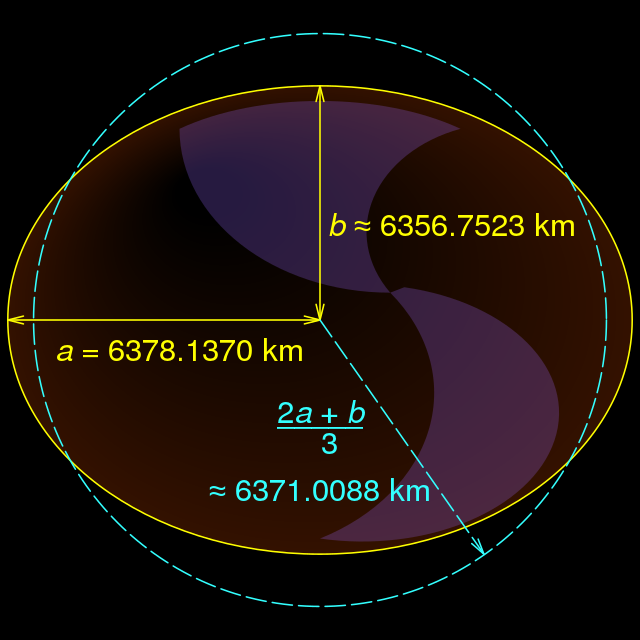
\includegraphics[width=0.8\textwidth]{Figures/Gravity/Exported/WGS84_mean_Earth_radius_Cmglee_Reversed.png}
    \tiny [Cmglee CCC 4.0]
\end{PointSix}
\end{frame}

% \begin{frame}
% \begin{PointSix}{Potential Fields}
%   \begin{itemize}
%     \item Rotation induces ellipsoidal shape approximate with reference ellipsoid.
%     \item Latitudinal correction of gravitation is adjusted accordingly.
%   \end{itemize}
% \end{PointSix}
% \end{frame}


\begin{frame}
  \begin{PointSix}{An ellipsoidal Earth}
      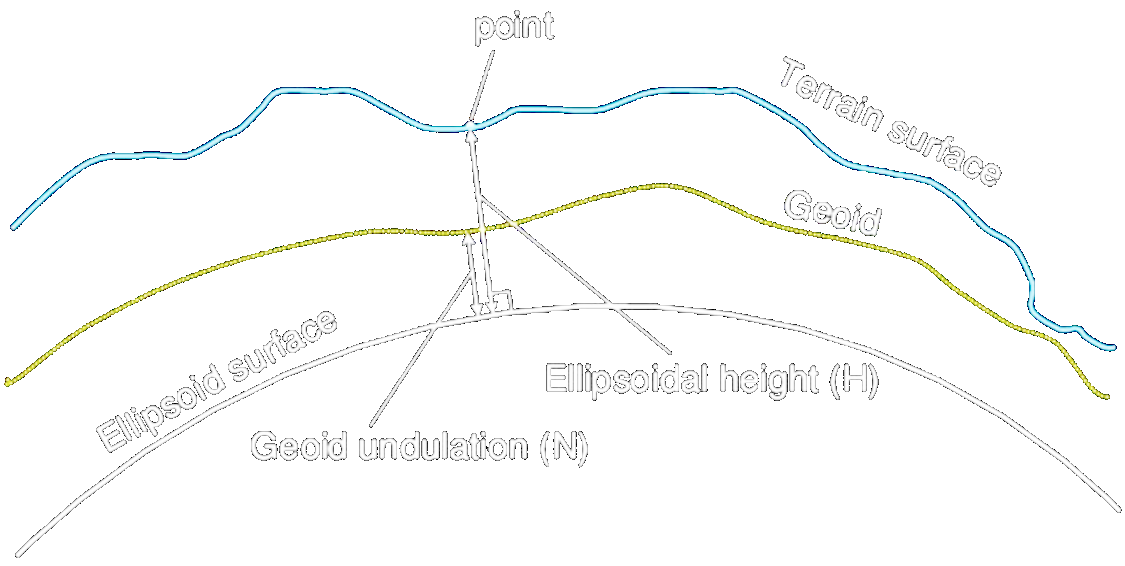
\includegraphics[width=0.9\textwidth]{Figures/Gravity/Exported/Geoid_Ziebart2004_TransparentBlack.png}

      \tiny [Ziebart et al., 2004] 

      \small
      \only<1>
      {
        \begin{itemize}
          \item Geoid is a real-world equipotential line approximating sea level.
          \item It is referenced to the geometric ellipsoid.
        \end{itemize}
      }
      \only<2>
      {
        \begin{itemize}
          \item The reference of elevation is a constant source of confusion.
          \item The geoid defines the local vertical direction.
        \end{itemize}
      }
      \only<3>
      {
        \begin{itemize}
          \item Upwarping of geoid indicates mass excess.
          \item Downwarping of geoid indicates mass deficit.
        \end{itemize}
      }
  \end{PointSix}
  \end{frame}


  \begin{frame}
    \begin{PointSix}{Learning Goals}
      \small
      \alert{Learning goals today:}
      \begin{itemize}
        \item Understand that gravity methods map sub-surface density variability
        \item Understand the gravitational force, its potential field, and one underlying measurement principle.
        \item Understand the Earth's geoid and reference ellipsoid
      \end{itemize}
    \end{PointSix}
    \end{frame}